\section{Integralrechnung}

\subsection{Fundamentalsatz und Stammfunktionen}

\begin{theorem}{Fundamentalsatz der Differential- und Integralrechnung}
    Seien $a<b$ und $f:[a,b] \to \R$ stetig.
    Die Funktion $F(x) = \int_{a}^{x} f(t) \dif t \quad a \leq x \leq b$ ist in $[a,b]$ stetig differenzierbar und $F'(x) = f(x) \quad \forall x \in [a,b]$.
\end{theorem}

\begin{definition}{Stammfunktion}
    Seien $a<b$ und $f:[a,b] \to \R$ stetig.
    Eine Funktion $F: [a,b] \to \R$ heisst \emph{Stammfunktion} von $f$, falls $F$ (stetig) differenzierbar in $[a,b]$ ist und $F' = f$ in $[a,b]$ gilt.

    Die Stammfunktion $F$ von $f$ ist bis auf eine additive Konstante eindeutig bestimmt und es gilt:
    \begin{equation}
        \int_{a}^{b} f(x) \dif x = F(b) - F(a)
    \end{equation}
\end{definition}

\begin{theorem}{Eigenschaften Integrierbarkeit}
    \begin{itemize}
        \item Sei $f : [a,b] \to \R$ \textit{stetig}. Dann ist $f$ integrierbar.
        \item Sei $f: [a,b] \to \R$ \textit{monoton}. Dann ist $f$ integrierbar.
        \item Seien $f,g : [a,b] \to \R$ beschränkt, integrierbar und $\lambda \in \R$.
                Dann sind $f+g$, $\lambda \cdot f$, $f \cdot g$, $|f|$, $\max(f,g)$ und $\frac{f}{g}$
                (falls $|g(x)| \geq \beta > 0 \quad \forall x \in [a,b]$) integrierbar.
        \item Seien $P,Q$ Polynome und $[a,b]$ ein Intervall, in dem $Q$ keine Nullstelle besitzt. Dann ist $[a,b] \to \R$, $x \mapsto \frac{P(x)}{Q(x)}$ integrierbar.
        \item Sind $f, g$ in einer endlichen Menge an Punkten verschieden, sind entweder beide oder keine der Beiden integrierbar.
        \item Sei $f: [a,b] \to \R$ stetig in dem kompakten Intervall $[a,b]$. Dann ist $f$ in $[a,b]$ gleichmässig stetig.
    \end{itemize}
\end{theorem}

\subsection{Unbestimmte und Bestimmte Integrale}

\begin{definition}{Unbestimmtes Integral}
    Sei $f: I \to \R$ auf einem Intervall $I \subseteq \R$ definiert.
    Falls $f$ stetig ist, gibt es eine Stammfunktion $F$ für $f$.
    \begin{equation}
        \int f(x) \dif x = F(x) + C
    \end{equation}
    Das unbestimmte Integral ist die Umkehroperation zur Ableitung.
\end{definition}

\begin{concept}{Integralregeln}
    \begin{itemize}
      \item Addition/Subtraktion:
      $$\int f(x-k) \dif x=F(x-k)+C$$
      \item Multiplikation:
      $$\int f(x \cdot k) \dif x=\frac{1}{k} F(x \cdot k)+C$$
      \item Skalarmultiplikation:
      $$\int \lambda_{1} f(x)+\lambda_{2} g(x) \dif x=\lambda_{1} F(x)+\lambda_{2} G(x)+C$$
    \end{itemize}
\end{concept}

\begin{definition}{Bestimmtes Integral}
    Für ein bestimmtes Integral von $f$ über $[a, b]$ schreibt man:
    \begin{equation}
        \int_{a}^{b} f(x) \dif x
    \end{equation}

    Sei $f(x)$ eine im Intervall $[a, b]$ stetige Funktion:
    \begin{equation}
        F'_{a}(x)=\frac{d}{dx}\left(\int_{a}^{x} f(t) \dif t\right)=f(x)
    \end{equation}

    Sei $f(x)$ eine im Intervall $[a, b]$ stetige Funktion, und sei $F(x)$ eine beliebige Stammfunktion von $f(x)$:
    \begin{equation}
        \int_{a}^{b} f(t) \dif t=F(b)-F(a)
    \end{equation}
\end{definition}

\begin{concept}{Rechnen mit bestimmten Integralen}
    Seien $a < b < c$ und $f: [a,b] \to \R$ beschränkt mit $f|_{[a,b]}$ und $f|_{[b,c]}$ integrierbar, sowie $\lambda_1, \lambda_2 \in \R$. Dann gilt:
    \begin{equation}
        \int_a^c f(x) \dif x = \int_a^b f(x) \dif x + \int_b^c f(x) \dif x
    \end{equation}
    und erweitert (mit Skalaren):
    \begin{equation}
        \int_a^b \left( \lambda_1 f_1 (x) + \lambda_2 f_2 (x) \right) \dif x = \lambda_1 \int_a^b f_1(x) \dif x + \lambda_2 \int_a^b f_2(x) \dif x
    \end{equation}
\end{concept}

\begin{definition}{Riemann-Integrale und Partitionen}
    Eine Partition von $[a,b]$ ist eine endliche Teilmenge $P \subseteq [a,b]$ wobei $\{a,b\} \subseteq P$.

    \textbf{Untersumme}: $s(f,P) \coloneqq \sum_{i=1}^n f_i \delta_i \qquad f_i = \inf\limits_{x_{i-1} \leq x \leq x_i} f(x)$

    \textbf{Obersumme}: $S(f,P) \coloneqq \sum_{i=1}^n F_i \delta_i \qquad F_i = \sup\limits_{x_{i-1} \leq x \leq x_i} f(x)$

    $\delta_i$ bezeichnet die Länge des Teilintervalls.
\end{definition}

\begin{lemma}{Verfeinerung und Menge P}
    \begin{enumerate}
        \item Sei $P'$ eine Verfeinerung von $P$, dann gilt:
            $s(f,P) \leq s (f,P') \leq S(f,P') \leq S(f, P)$
        \item Für beliebige Partitionen $P_1, P_2$ gilt: $s(f,P_1) \leq S(f,P_2)$.
    \end{enumerate}
\end{lemma}

\begin{definition}{Riemann Integrierbar}
    Eine beschränkte Funktion $f : [a,b] \to \R$ ist Riemann integrierbar, falls $s(f) = S(f)$. In diesem Fall bezeichnen wir den gemeinsamen Wert von $s(f)$ und $S(f)$ mit
    $\int_{a}^{b} f(x) \dif x$

    Sei $\mathcal{P}(I)$ die Menge der Partitionen von $I$:
    \begin{equation}
        s(f) = \sup_{P \in \mathcal{P}(I)} s(f,P) \qquad S(f) = \inf_{P \in \mathcal{P}(I)} S(f,P)
    \end{equation}
\end{definition}

\begin{theorem}{Alternative Kriterien}
    Eine beliebige beschränkte Funktion $f$ ist genau dann integrierbar, falls:
    \begin{itemize}
         \item $\forall \varepsilon > 0 ~ \exists P \in \mathcal{P}(I) \quad \text{mit} \quad S(f,P) - s(f,P) < \varepsilon$
    \end{itemize}

    Für $f : [a,b] \to \R$:
    \begin{itemize}
         \item $\forall \varepsilon > 0 ~\exists \delta > 0$ sodass
    $\forall P \in \mathcal{P}_\delta (I), S(f,P) - s(f,P) < \varepsilon$
     \end{itemize}

    Mit $A \coloneqq \int_a^b f(x) \dif x$:
    \begin{itemize}
        \item $\forall \varepsilon > 0 ~ \exists \delta > 0$ sodass $\forall P \in \mathcal{P} (I)$ Partition mit $\delta(P) < \delta$ und $\xi_1 , \ldots , \xi_n$ mit $\xi_i \in [x_{i-1},x_i]$, $P = \{x_0 , \ldots , x_n\}$ gilt:
        $$\left| A - \sum_{i=1}^n f(\xi_i) (x_i - x_{i-1})\right| < \varepsilon$$
    \end{itemize}
\end{theorem}

\subsection{Wichtige Stammfunktionen}

\begin{highlight}{Wichtige Stammfunktionen}
    $\int f(x) \dif x \Longrightarrow F(x) + C$
    \begin{center}
        \begin{minipage}{0.45\linewidth}
            \tcbsubtitle{Potenzfunktionen}
            \begin{align*}
                &\int x^n \dif x  &=&  \quad \frac{1}{n+1}x^{n+1} \quad (n \neq -1) \\
                &\int \frac{f'}{f} \dif x  &=&  \quad \ln \left\lvert f \right\rvert  \\
                &\int \frac{1}{x} \dif x  &=& \quad \ln \left\lvert x \right\rvert  \\
                &\int \frac{1}{x+a} \dif x  &=&  \quad \ln \left\lvert x+a \right\rvert \\
                &\int \frac{1}{(x+a)^2} \dif x  &=&  -\frac{1}{x+a}  \\
                &\int \frac{1}{\sqrt{x}}\dif x  &=&  2 \sqrt{x}  \\
            \end{align*}
        \end{minipage}
        \hfill\vline\hfill
        \begin{minipage}{0.45\linewidth}
            \tcbsubtitle{Exponential- und Logarithmusfunktionen}
            \begin{align*}
                &\int e^{x} \dif x  &=& e^{x} \\
                &\int e^{ax} \dif x  &=&  \frac{1}{a} e^{ax}  \\
                &\int a^{x} \dif x \quad  &=& \frac{a^{x}}{\ln (a)} \\
                &\int \ln (x) \dif x  &=& x \cdot \ln (x)-x \\
                &\int \log_{a}(x) \dif x  &=& \frac{x \cdot \ln (x)-x}{\ln (a)} \\
            \end{align*}
        \end{minipage}
    \end{center}

    \tcbsubtitle{Trigonometrische Funktionen}
    \begin{center}
        \begin{minipage}{0.4\linewidth}
            \begin{align*}
                &\int\cos (x) \dif x  &=& \sin (x) \\
                &\int\sin (x) \dif x  &=& -\cos (x) \\
                &\int\tan (x) \dif x  &=& -\ln |\cos (x)| \\
                &\int \sin(ax)\dif x  &=&  - \frac{1}{a} \cos(a x)  \\
                &\int \sin^2(ax)\dif x  &=&  \frac{x}{2} - \frac{1}{4a} \sin(2 a x)  \\
                &\int \cos(ax)\dif x  &=&  \frac{1}{a} \sin(a x)  \\
                &\int \cos^2(ax)\dif x  &=&  \frac{x}{2} + \frac{1}{4a} \sin(2 a x)  \\
            \end{align*}
        \end{minipage}
        \hfill\vline\hfill
        \begin{minipage}{0.45\linewidth}
            \begin{align*}
                &\int\frac{1}{1+x^{2}} \dif x  &=& \arctan (x)\\
                &\int\frac{1}{\sqrt{1-x^{2}}} \dif x  &=& \arcsin (x) \\
                &\int -\frac{1}{\sqrt{1-x^{2}}} \dif x  &=& \arccos (x) \\
            \end{align*}
        \end{minipage}
    \end{center}
\end{highlight}

\subsection{Rechnen mit Integralen}

\begin{corollary}{Nützliche Regeln}
    Sei $I \subseteq \R$ ein Intervall und $f: I \to \R$ stetig.
    \begin{enumerate}
        \item Seien $a,b,c \in \R$, sodass das abgeschlossene Intervall mit den Endpunkten $a+c$, $b+c$ in $I$ enthalten ist.
            Dann gilt
            \begin{equation}
                \int_{a+c}^{b+c} f(x) \dif x = \int_{a}^{b} f(t+c) \dif t
            \end{equation}
        \item Seien $a,b,c \in \R$ mit $c \neq 0$, sodass das abgeschlossene Intervall mit Endpunkten $ac$, $bc$ in $I$ enthalten ist.
            Dann gilt
            \begin{equation}
                \int_{a}^{b} f(ct) \dif t = \frac{1}{c} \int_{ac}^{bc} f(x) \dif x
            \end{equation}
    \end{enumerate}
\end{corollary}

\begin{concept}{Symmetrie ungerader Funktionen}
    Falls eine Funktion ungerade ist und symmetrische Grenzen hat:
    \begin{equation}
        \int_{-a}^{a} f(x) \dif x = 0 \quad \text{für ungerade } f
    \end{equation}

    Beispiel: $\int_{-\frac{\pi}{2}}^{\frac{\pi}{2}} (\sin x)^7 \cos x \dif x = 0$
\end{concept}

\begin{KR}{Flächeninhalt bei wechselndem Vorzeichen von $f(x)$}
    \begin{itemize}
      \item $[a, b]$ = Intervall
      \item $x_{1}, x_{2}, \ldots, x_{n}$ = Nullstellen
    \end{itemize}

    $$\left|\int_{a}^{x_{1}} f(x) \dif x\right|+\left|\int_{x_{1}}^{x_{2}} f(x) \dif x\right|+\cdots+\left|\int_{x_{n}}^{b} f(x) \dif x\right|$$
\end{KR}

\begin{center}
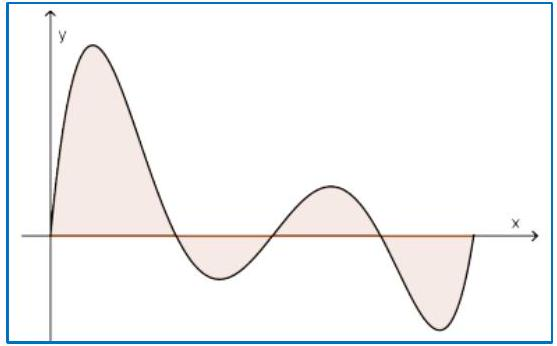
\includegraphics[scale=0.25]{2024_01_20_7bfda6c084929ccc01ffg-06(1).jpg}
\end{center}

\begin{KR}{Flächeninhalt zwischen zwei Kurven $f(x)$ und $g(x)$}
    \begin{itemize}
      \item $[a, b]$ = Intervall
      \item $x_{1}, x_{2}, \ldots, x_{n}$ = Schnittpunkte
    \end{itemize}
    $$\left|\int_{a}^{x_{1}}(f(x)-g(x)) \dif x\right|+\left|\int_{x_{1}}^{x_{2}}(f(x)-g(x)) \dif x\right|+\cdots+\left|\int_{x_{n}}^{b}(f(x)-g(x)) \dif x\right|$$
\end{KR}

\begin{center}
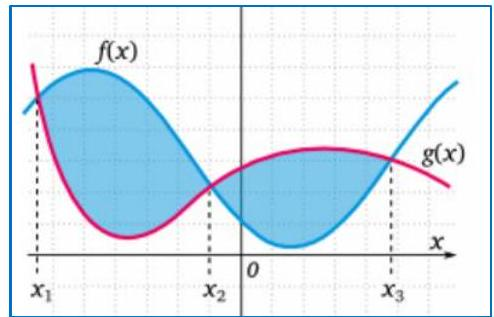
\includegraphics[scale=0.25]{2024_01_20_7bfda6c084929ccc01ffg-06(2).jpg}
\end{center}

\begin{KR}{Strategie zur Berechnung von Integralen}
    \textbf{Bruchform:}
    \begin{enumerate}
        \item Vereinfache, so dass ein einfacher Nenner entsteht
        \item Partialbruchzerlegung
        \item $\frac{u'}{2\sqrt{u}}$ oder $\frac{u'}{u}$ erkennen $\Rightarrow \sqrt{u}$ oder $\ln|u|$
    \end{enumerate}

    \textbf{Produktform:}
    \begin{enumerate}
        \item Partielle Integration anwenden (evtl. mehrmals)
        \item Kettenregel verwenden
    \end{enumerate}

    \textbf{Potenzen:}

    $\int_{a}^{b} f(x)^{c} \dif x$ umformen in $\int_{a}^{b}\left(f(x)^{c} \cdot 1\right) \dif x$ oder $\int_{a}^{b}\left(f(x)^{c-1} \cdot f(x)\right) \dif x$ um dann partielle Integration anzuwenden

    \textbf{Exponentenform:}

    $e / \log$ Trick verwenden, wenn Variable im Exponenten ist.

    \textbf{Produkt mit $e, \sin , \cos$:}

    Mehrmals partielle Integration anwenden, wobei sin, cos immer $g'$ und immer $f$ ist.

    \textbf{Summe im Integral:}

    Summe aus dem Integral herausziehen (dafür muss die Reihe gleichmässig konvergieren)
\end{KR}

\begin{corollary}{Ungleichungen}
    Seien $f,g : [a,b] \to \R$ beschränkt integrierbar:
    \begin{enumerate}
        \item $f(x) \leq g(x) \quad \forall x \in [a,b]$ $\Rightarrow$ $\int_a^b f(x) \dif x \leq \int_a^b g(x) \dif x$
        \item $\left| \int_a^b f(x) \dif x \right| \leq \int_a^b |f(x)| \dif x$
        \item $\left| \int_a^b f(x) g(x) \dif x \right| \leq \sqrt{\int_{a}^{b} f^2(x) \dif x} \sqrt{\int_{a}^{b} g^2(x) \dif x}$
    \end{enumerate}
\end{corollary}

\begin{theorem}[important]{Mittelwertsatz}
    Sei $f:[a,b] \to \R$ stetig.
    Dann gibt es $\xi \in [a,b]$ mit
    \begin{equation}
        \int_{a}^{b} f(x) \dif x = f(\xi)(b-a)
    \end{equation}
\end{theorem}

\begin{theorem}{Folgerung Mittelwertsatz}
    Seien $f,g: [a,b] \to \R$ wobei $f$ stetig, $g$ beschränkt integrierbar mit $g(x) \geq 0~\forall x \in [a,b]$.
    Dann gibt es $\xi \in [a,b]$ mit
    \begin{equation}
        \int_{a}^{b} f(x)g(x) \dif x = f(\xi) \int_{a}^{b} g(x) \dif x
    \end{equation}
\end{theorem}

\subsection{Partielle Integration}

\begin{concept}{Partielle Integration}
    Seien $a < b$ reelle Zahlen und $f,g:[a,b] \to \R$ stetig differenzierbar. Dann gilt
    \begin{equation}
        \int_a^b f(x) g'(x) \dif x = f(b) g(b) - f(a) g(a) - \int_a^b f'(x)g(x) \dif x
    \end{equation}
    bzw. für unbestimmte Integrale
    \begin{equation}
        \int f(x) \cdot g'(x) \dif x = f(x) \cdot g(x) - \int f'(x) \cdot g(x) \dif x
    \end{equation}
\end{concept}

\begin{KR}{Prioritäten für partielle Integration}
    Für die partielle Integration $f(x)$ nach folgender Priorität auswählen:
    \begin{center}
    \begin{tabular}{lll}
        1. $\log_e, \log_a$  &  3. $x^2, 5x^3$ & 5. $e^x, 5a^x$\\
        2. $\arcsin, \arccos$ & 4. $\sin, \cos, \tan$ &
    \end{tabular}
    \end{center}
\end{KR}

\begin{remark}
    $\uparrow$ 1 falls arc- oder log-Funktion vorkommt, $x^{n}, \frac{1}{1-x^{2}}, \frac{1}{1+x^{2}}$

    $\downarrow$ $x^{n}, \arcsin (x), \arccos (x), \arctan (x)$
\end{remark}

\subsection{Substitution}

\begin{concept}{Substitution}
    Die Substitution ist die Umkehrung der Kettenregel. D.h. wir wollen Substitution vorallem verwenden, wenn wir innere Funktionen haben.
    \begin{equation}
        \int_{a}^{b} f(g(t)) g'(t) \dif t = \int_{g(a)}^{g(b)} f(x) \dif x
    \end{equation}
    bzw. für unbestimmte Integrale
    \begin{equation}
        \int f(g(t)) \cdot g'(t) \dif t=\left.\int f(x) \dif x\right|_{x=g(t)}
    \end{equation}
\end{concept}

\begin{formula}{Nützliche Substitutionen}
    \begin{itemize}
        \item $e^{x}, \sinh (x), \cosh (x)$, subst: $t=e^{a x}, \dif x=\frac{\dif t}{a t}$. Dann $\sinh = \cosh = \frac{t^{2}-1}{2 t}$
        \item $\log (x)$ subst: $t=\log (x), x=e^{t}, \dif x=e^{t} \dif t$
        \item für gerade $n: \cos^{n}(x), \sin^{n}(x), \tan (x)$ Sub: $t=\tan (x)$, $\dif x=\frac{1}{1+t^{2}} \dif t, \sin^{2}(x)=\frac{t^{2}}{1+t^{2}}, \cos^{2}(x)=\frac{1}{1+t^{2}}$
        \item für ungerade $n: \cos^{n}(x), \sin^{n}(x)$, Sub: $t=\tan (x / 2)$, $\dif x=\frac{2}{1+t^{2}} \dif t, \sin (x)=\frac{2 t}{1+t^{2}}, \cos (x)=\frac{1-t^{2}}{1+t^{2}}$
        \item $\int \sqrt{1-x^{2}} \dif x$ sub: $x=\sin (x)$ oder $\cos (x)$
        \item $\int \sqrt{1+x^{2}} \dif x$ sub: $x=\sinh (x)$
    \end{itemize}
\end{formula}

\begin{example}
    Bsp. $\int \frac{x}{\sqrt{9-x^{2}}} \dif x$ substitution mit $t=\sqrt{9-x^{2}}$.

    $$\Rightarrow x=\sqrt{9-t^{2}} \Rightarrow x'=\frac{-2 t}{2 \sqrt{9-t^{2}}} \Rightarrow \dif x=\frac{-t \cdot \dif t}{\sqrt{9-t^{2}}}$$

    $\int-\dif t=-t$ rücksubstitution $\Rightarrow-\sqrt{9-x^{2}}$
\end{example}

\subsection{Partialbruchzerlegung}

\begin{KR}{Stammfunktionen rationaler Funktionen}
    Die Stammfunktion einer Funktion $R(x)=\frac{P(x)}{Q(x)}$ bestehend aus rationalen Funktionen lässt sich als eine Funktion von Polynomen, rationalen, exponentiellen, logarithmischen, trigonometrischen und inversen trigonometrischen Funktionen darstellen.

    Zuerst wollen wir, dass $\grad(P)<\grad(Q)$ gilt, falls dies nicht der Fall ist, führen wir Polynomdivision aus. Danach bestimmen wir alle reellen und komplexen Nullstellen. Nun gilt:

    $$R(x)=\sum_{k=1}^{N} R_{k}(x)+\sum_{k=1}^{M} Q_{k}(x)$$

    Hier ist $N$ die Anzahl reeller Nullstellen und $M$ die Anzahl der komplexen Nullstellen. Es gilt:

    $$\begin{gathered}
    R_{k}(x)=\frac{a_{k_{1}}}{(x-x_{k})}+\frac{a_{k_{2}}}{(x-x_{k})^{2}}+\ldots+\frac{a_{k_{n_{k}}}}{(x-x_{k})^{n_{k}}} \\
    Q_{k}(x)=\frac{a_{k_{1}}+b_{k_{1}} x}{((x-\alpha_{k})^{2}+\beta_{k}^{2})}+\ldots+\frac{a_{k_{m_{k}}}+b_{k_{m_{k}}} x}{((x-\alpha_{k})^{2}+\beta_{k}^{2})^{m_{k}}}
    \end{gathered}$$

    Somit können wir die Funktion mit Partialbruchzerlegung in einzelne Brüche darstellen, welche dann leichter zu integrieren sind. Wenn wir eine reelle Nullstelle haben, so gilt:

    $$\int \frac{1}{(x-\gamma_{i})^{n}} \dif x =\begin{cases}
    \ln (x-\gamma_{i}) & \text{für } n=1 \\
    \frac{-1}{(n-1)(x-\gamma_{i})^{n-1}} & \text{für } n > 1
    \end{cases}$$

    Für komplexe Nullstellen gilt:

    $$\begin{gathered}
    \frac{A+B x}{((x-\alpha)^{2}+\beta^{2})^{j}}=\frac{B(x-\alpha)}{((x-\alpha)^{2}+\beta^{2})^{j}}+\frac{A+B \alpha}{((x-\alpha)^{2}+\beta^{2})^{j}} \\
    \int \frac{B(x-\alpha)}{((x-\alpha)^{2}+\beta^{2})^{j}} \dif x =\begin{cases}
    \frac{B}{2} \ln ((x-\alpha)^{2}+\beta^{2}) & \text{für } j=1 \\
    \frac{B}{(2(1-j))((x-\alpha)^{2}+\beta^{2})^{j-1}} & \text{für } j > 1
    \end{cases}
    \end{gathered}$$

    Für den letzten Term brauchen wir die Substitution $(x-\alpha)=\beta t$:

    $$\int \frac{A+B \alpha}{((x-\alpha)^{2}+\beta^{2})^{j}} \dif x=\frac{A+B \alpha}{\beta^{2 j-1}} \cdot \int \frac{1}{(t^{2}+1)^{j}} \dif t$$
\end{KR}

\begin{example}
    Bsp.
    $$\int \frac{x^{2}-x+2}{x^{3}-x^{2}+x-1} \dif x$$

    Wir finden die erste Nullstelle $(x-1)$ durch Ausprobieren. Danach führen wir Polynomdivision (durch $x-1$) aus und erhalten damit die weitere Nullstelle $(x^{2}+1)$. Da $x^{2}+1$ eine komplexe Nullstelle ist, nehmen wir dafür $A+B x$:

    $$\frac{A+B x}{x^{2}+1}+\frac{C}{x-1}=\frac{x^{2}-x+2}{(x^{2}+1)(x-1)}$$

    $\Longrightarrow x^{2}-x+2=(A+C) \cdot x^{2}+(B-A) x+(C-B) \cdot 1$

    $\Longrightarrow B=0, A=-1, C=1$

    $\Longrightarrow \int \frac{1}{x-1}+\frac{-1}{x^{2}+1} \dif x=\ln (x-1)-\arctan (x)+C$
\end{example}

\begin{corollary}{Reduktionsformel}
    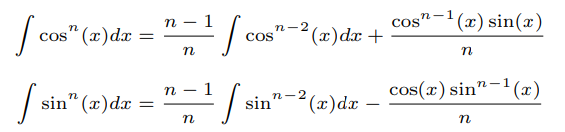
\includegraphics[scale=0.5]{reduktionsformel.png}
\end{corollary}

\subsection{Uneigentliche Integrale und weitere Themen}

\begin{theorem}[important]{Euler-McLaurin Summenformel}
    Wird verwendet, um Summen (wie $\sum_{i=1}^n \frac{1}{i}$, $\sum_{i=1}^n \ln{i}$ oder $\sum_{i=1}^n i^\ell$) abzuschätzen.

    Sei $f : [0,n] \to \R$ $k$-mal stetig differenzierbar, $k \geq 1$.
    Dann gilt:
    \begin{enumerate}
        \item Für $k=1$:
        \begin{equation}
            \sum^{n}_{i=1} f(i) = \int_{0}^{n} f(x) \dif x + \frac{1}{2} ( f(n) - f(0) ) + \int_{0}^{n} \tilde{B}_1 (x) f'(x) \dif x
        \end{equation}
        \item Für $k \geq 2$:
        \begin{align}
            \sum^{n}_{i=1} f(i) &= \int_{0}^{n} f(x) \dif x + \frac{1}{2} ( f(n) - f(0) )\\
            &+ \sum^{k}_{j=2} \frac{(-1)^j B_j}{j!} ( f^{(j-1)} (n) - f^{(j-1)} (0) ) + \tilde{R}_k
        \end{align}
        wobei $\tilde{R}_k = \frac{(-1)^{k-1}}{k!} \int_{0}^{n} \tilde{B}_k (x) f^{(k)} (x) \dif x$
    \end{enumerate}
\end{theorem}

\begin{highlight}{Potenzsummen}
    Für Potenzsummen der Form $1^l + 2^l + \ldots + n^l$ wobei $l \geq 1, l \in \N$ kann die Summenformel mit $f(x) = x^l$ und $k=l+1$ angewendet werden.
    Daraus folgt für alle $l \geq 1$:
    \begin{equation}
        1^l + 2^l + \ldots + n^l = \frac{1}{l+1} \sum^{l}_{j=0} (-1)^j \begin{pmatrix}l+1\\j\end{pmatrix} B_j n^{l+1-j}
    \end{equation}
\end{highlight}

\begin{concept}{Integration konvergenter Reihen}
    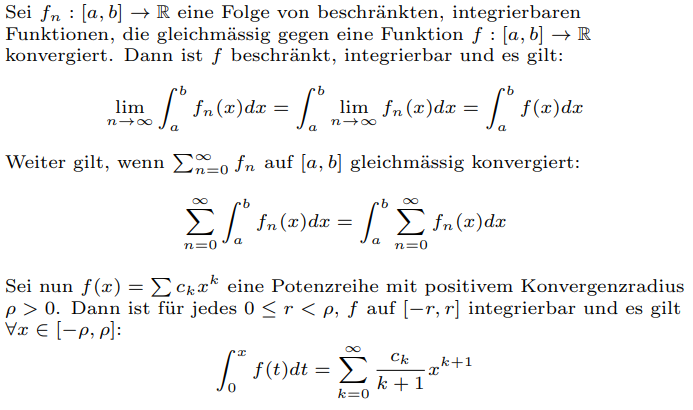
\includegraphics[scale=0.5]{integration_konvergenter_reihen.png}
\end{concept}

\begin{lemma}{Holder'sche Ungleichung}
    Sei $p > 1$ und $q > 1$ mit $\frac{1}{p} + \frac{1}{q} =1$.
    Dann gilt $\forall a,b \geq 0$:
    \begin{equation}
        a \cdot b \leq \frac{a^p}{p} + \frac{b^q}{q}
    \end{equation}
\end{lemma}

\begin{theorem}{Verallgemeinerung Holder'sche Ungleichung}
    Seien $p > 1$ und $q> 1$ mit $\frac{1}{p} + \frac{1}{q} = 1$.
    Für alle $f,g : [a,b] \to \R$ stetig gilt:
    \begin{equation}
        \int_{a}^{b} |f(x) g(x)| \dif x \leq ||f||_p ||g||_q
    \end{equation}
    wobei $||f||_p \coloneqq \left( \int_{a}^{b} |f(x)|^p \dif x \right)^{\frac{1}{p}}$
\end{theorem}
